\documentclass[11pt]{article}
\usepackage[margin=1in]{geometry}
\usepackage{graphicx}
\usepackage{booktabs}
\usepackage{hyperref}
\usepackage{amsmath}
\usepackage{float}
\usepackage{multirow}

\title{\textbf{Detecting Boilerplate Responses in LLMs via First-Token Log-Probabilities}}
\author{Yasser BOUHAI}
\date{\today}

\begin{document}

\maketitle

\section{Introduction}

This work implements the methodology from \textit{"Do Stop Me Now: Detecting Boilerplate Responses with a Single Iteration"} by Kainan and Zychlinski. The paper demonstrates that large language models encode their intent in the log-probability distribution of the first generated token, enabling proactive detection of boilerplate responses—including refusals, greetings, and gratitude expressions—before any text generation occurs.

\subsection{Motivation}

Traditional response classification requires generating model output and analyzing the text, wasting computational resources. This approach detects boilerplate response types \textbf{before generation} by examining only the first token's log-probabilities, offering:

\begin{itemize}
    \item \textbf{Proactive boilerplate detection} --- Identify response type before wasting compute on full generation
    \item \textbf{Multi-class intent classification} --- Distinguish between chat responses, greetings, thanks, and refusals
    \item \textbf{Computational efficiency} --- Classification takes milliseconds after one-time feature extraction
    \item \textbf{Early termination/routing} --- Route simple responses to smaller models or skip generation entirely
\end{itemize}

\section{Methodology}

\subsection{Dataset}

The \texttt{jfrog/boilerplate-detection} dataset contains 2,906 samples across 4 categories:
\begin{itemize}
    \item \textbf{Chat} (53.7\%): Normal conversation responses
    \item \textbf{Refusal} (35.6\%): Model refusing to answer
    \item \textbf{Thanks} (9.8\%): Gratitude expressions
    \item \textbf{Hello} (0.9\%): Greeting messages
\end{itemize}

\subsection{Feature Extraction}

For each input prompt, we extract the log-probability distribution over the entire vocabulary for the first token. This produces a high-dimensional vector (150K--260K dimensions depending on model vocabulary size).

\subsection{Dimensionality Reduction}

Due to hardware constraints (NVIDIA RTX 3060 Laptop GPU), we apply variance-based feature selection to reduce dimensionality from $\sim$150K to 1,000 features by selecting the top-1,000 tokens with highest variance across samples.

\subsection{Classification}

We use k-Nearest Neighbors (k=3) with cosine distance for classification. The model is evaluated using 5-fold stratified cross-validation to ensure robust performance estimates.

\subsection{Implementation Constraints}

Unlike the original paper which uses full-precision models, this implementation uses:
\begin{itemize}
    \item \textbf{8-bit quantization (INT8)} via bitsandbytes library
    \item \textbf{Variance-based feature selection} (1,000 from 150K+ dimensions)
    \item \textbf{Memory-efficient k-NN} with batched distance computation
\end{itemize}

These optimizations allow the experiments to run on consumer hardware while maintaining usable performance.

\section{Results}

\subsection{Overall Performance}

the following table compares our results with the original paper. Despite using 8-bit quantization and reduced feature space, the models achieve 76--79\% F1-scores, approximately 20\% lower than the paper's full-precision results.

\begin{table}[H]
\centering
\caption{Model Performance (5-Fold Cross-Validation)}
\label{tab:overall}
\begin{tabular}{@{}lcccc@{}}
\toprule
\textbf{Model} & \textbf{Accuracy} & \textbf{Precision} & \textbf{Recall} & \textbf{F1-Score} \\
\midrule
Qwen2.5-1.5B (8-bit) & 0.816 & 0.817 & 0.774 & 0.788 \\
Llama-3.2-3B (8-bit) & 0.801 & 0.803 & 0.749 & 0.768 \\
Gemma-3-1B (8-bit) & 0.820 & 0.835 & 0.770 & 0.789 \\
\midrule
\textit{Paper: Qwen2.5-1.5B} & \textit{0.997} & \textit{0.991} & \textit{0.998} & \textit{0.994} \\
\textit{Paper: Llama-3.2-3B} & \textit{0.995} & \textit{0.996} & \textit{0.984} & \textit{0.990} \\
\textit{Paper: Gemma-3-1B} & \textit{0.994} & \textit{0.997} & \textit{0.997} & \textit{0.997} \\
\bottomrule
\end{tabular}
\end{table}

\subsection{Per-Category Performance}

The table  shows detailed metrics for each response type. Key observations:
\begin{itemize}
    \item \textbf{Hello} messages are detected perfectly or near-perfectly (F1: 0.96--1.00)
    \item \textbf{Chat} responses are reliably classified (F1: 0.87--0.88)
    \item \textbf{Refusal} detection remains strong despite quantization (F1: 0.76--0.79)
    \item \textbf{Thanks} messages are harder to classify due to limited samples (only 9.8\% of dataset)
\end{itemize}

\begin{table}[H]
\centering
\caption{Per-Category Performance (Combined Cross-Validation)}
\label{tab:category}
\begin{tabular}{@{}llccc@{}}
\toprule
\textbf{Model} & \textbf{Category} & \textbf{Precision} & \textbf{Recall} & \textbf{F1-Score} \\
\midrule
\multirow{4}{*}{Qwen2.5-1.5B} & Chat & 0.87 & 0.90 & 0.88 \\
 & Hello & 1.00 & 1.00 & 1.00 \\
 & Refusal & 0.77 & 0.79 & 0.78 \\
 & Thanks & 0.63 & 0.40 & 0.49 \\
\midrule
\multirow{4}{*}{Llama-3.2-3B} & Chat & 0.85 & 0.90 & 0.87 \\
 & Hello & 1.00 & 0.93 & 0.96 \\
 & Refusal & 0.76 & 0.77 & 0.76 \\
 & Thanks & 0.59 & 0.40 & 0.48 \\
\midrule
\multirow{4}{*}{Gemma-3-1B} & Chat & 0.85 & 0.92 & 0.88 \\
 & Hello & 1.00 & 1.00 & 1.00 \\
 & Refusal & 0.79 & 0.78 & 0.79 \\
 & Thanks & 0.69 & 0.38 & 0.49 \\
\bottomrule
\end{tabular}
\end{table}

\subsection{t-SNE Visualizations}

The next 3 Figures show 2D t-SNE projections of the 1,000-dimensional feature vectors. Clear cluster separation demonstrates that models encode intent classification information in the first token's probability distribution.

\begin{figure}[H]
\centering
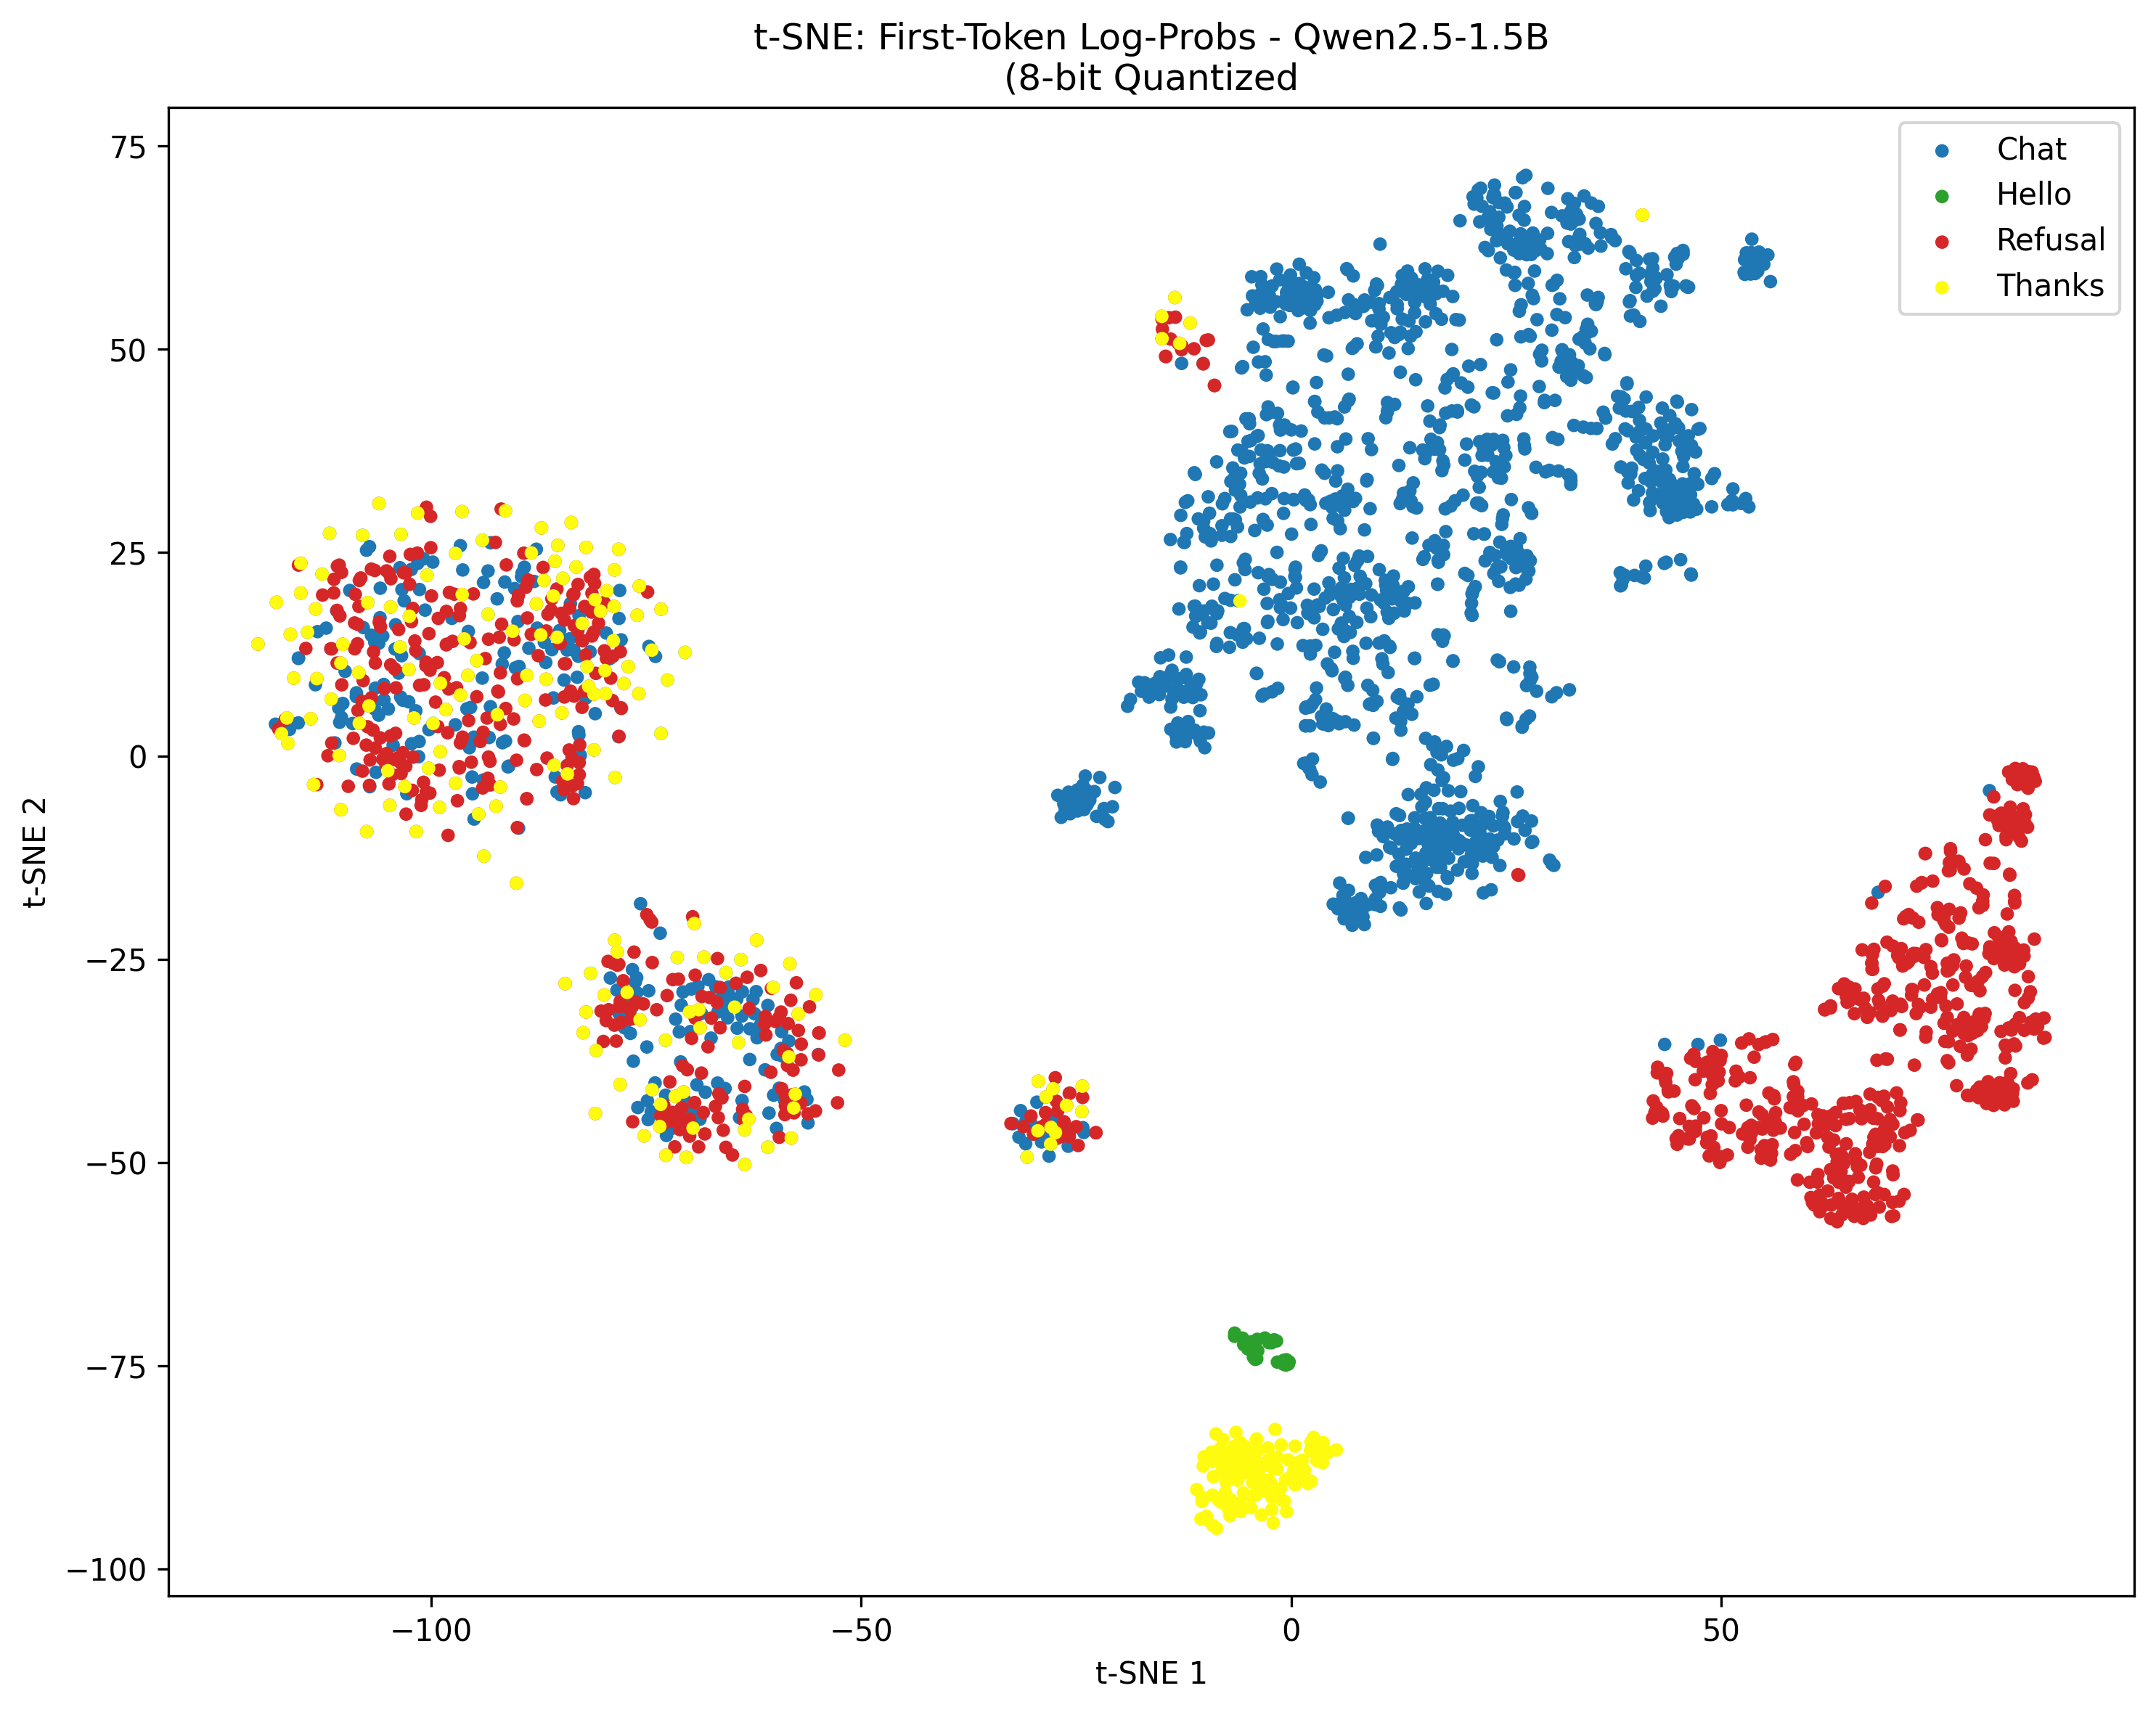
\includegraphics[width=0.7\textwidth]{tsne_Qwen2_5_1_5B_8bit.png}
\caption{Qwen2.5-1.5B: t-SNE visualization of first-token log-probabilities}
\label{fig:qwen}
\end{figure}

\begin{figure}[H]
\centering
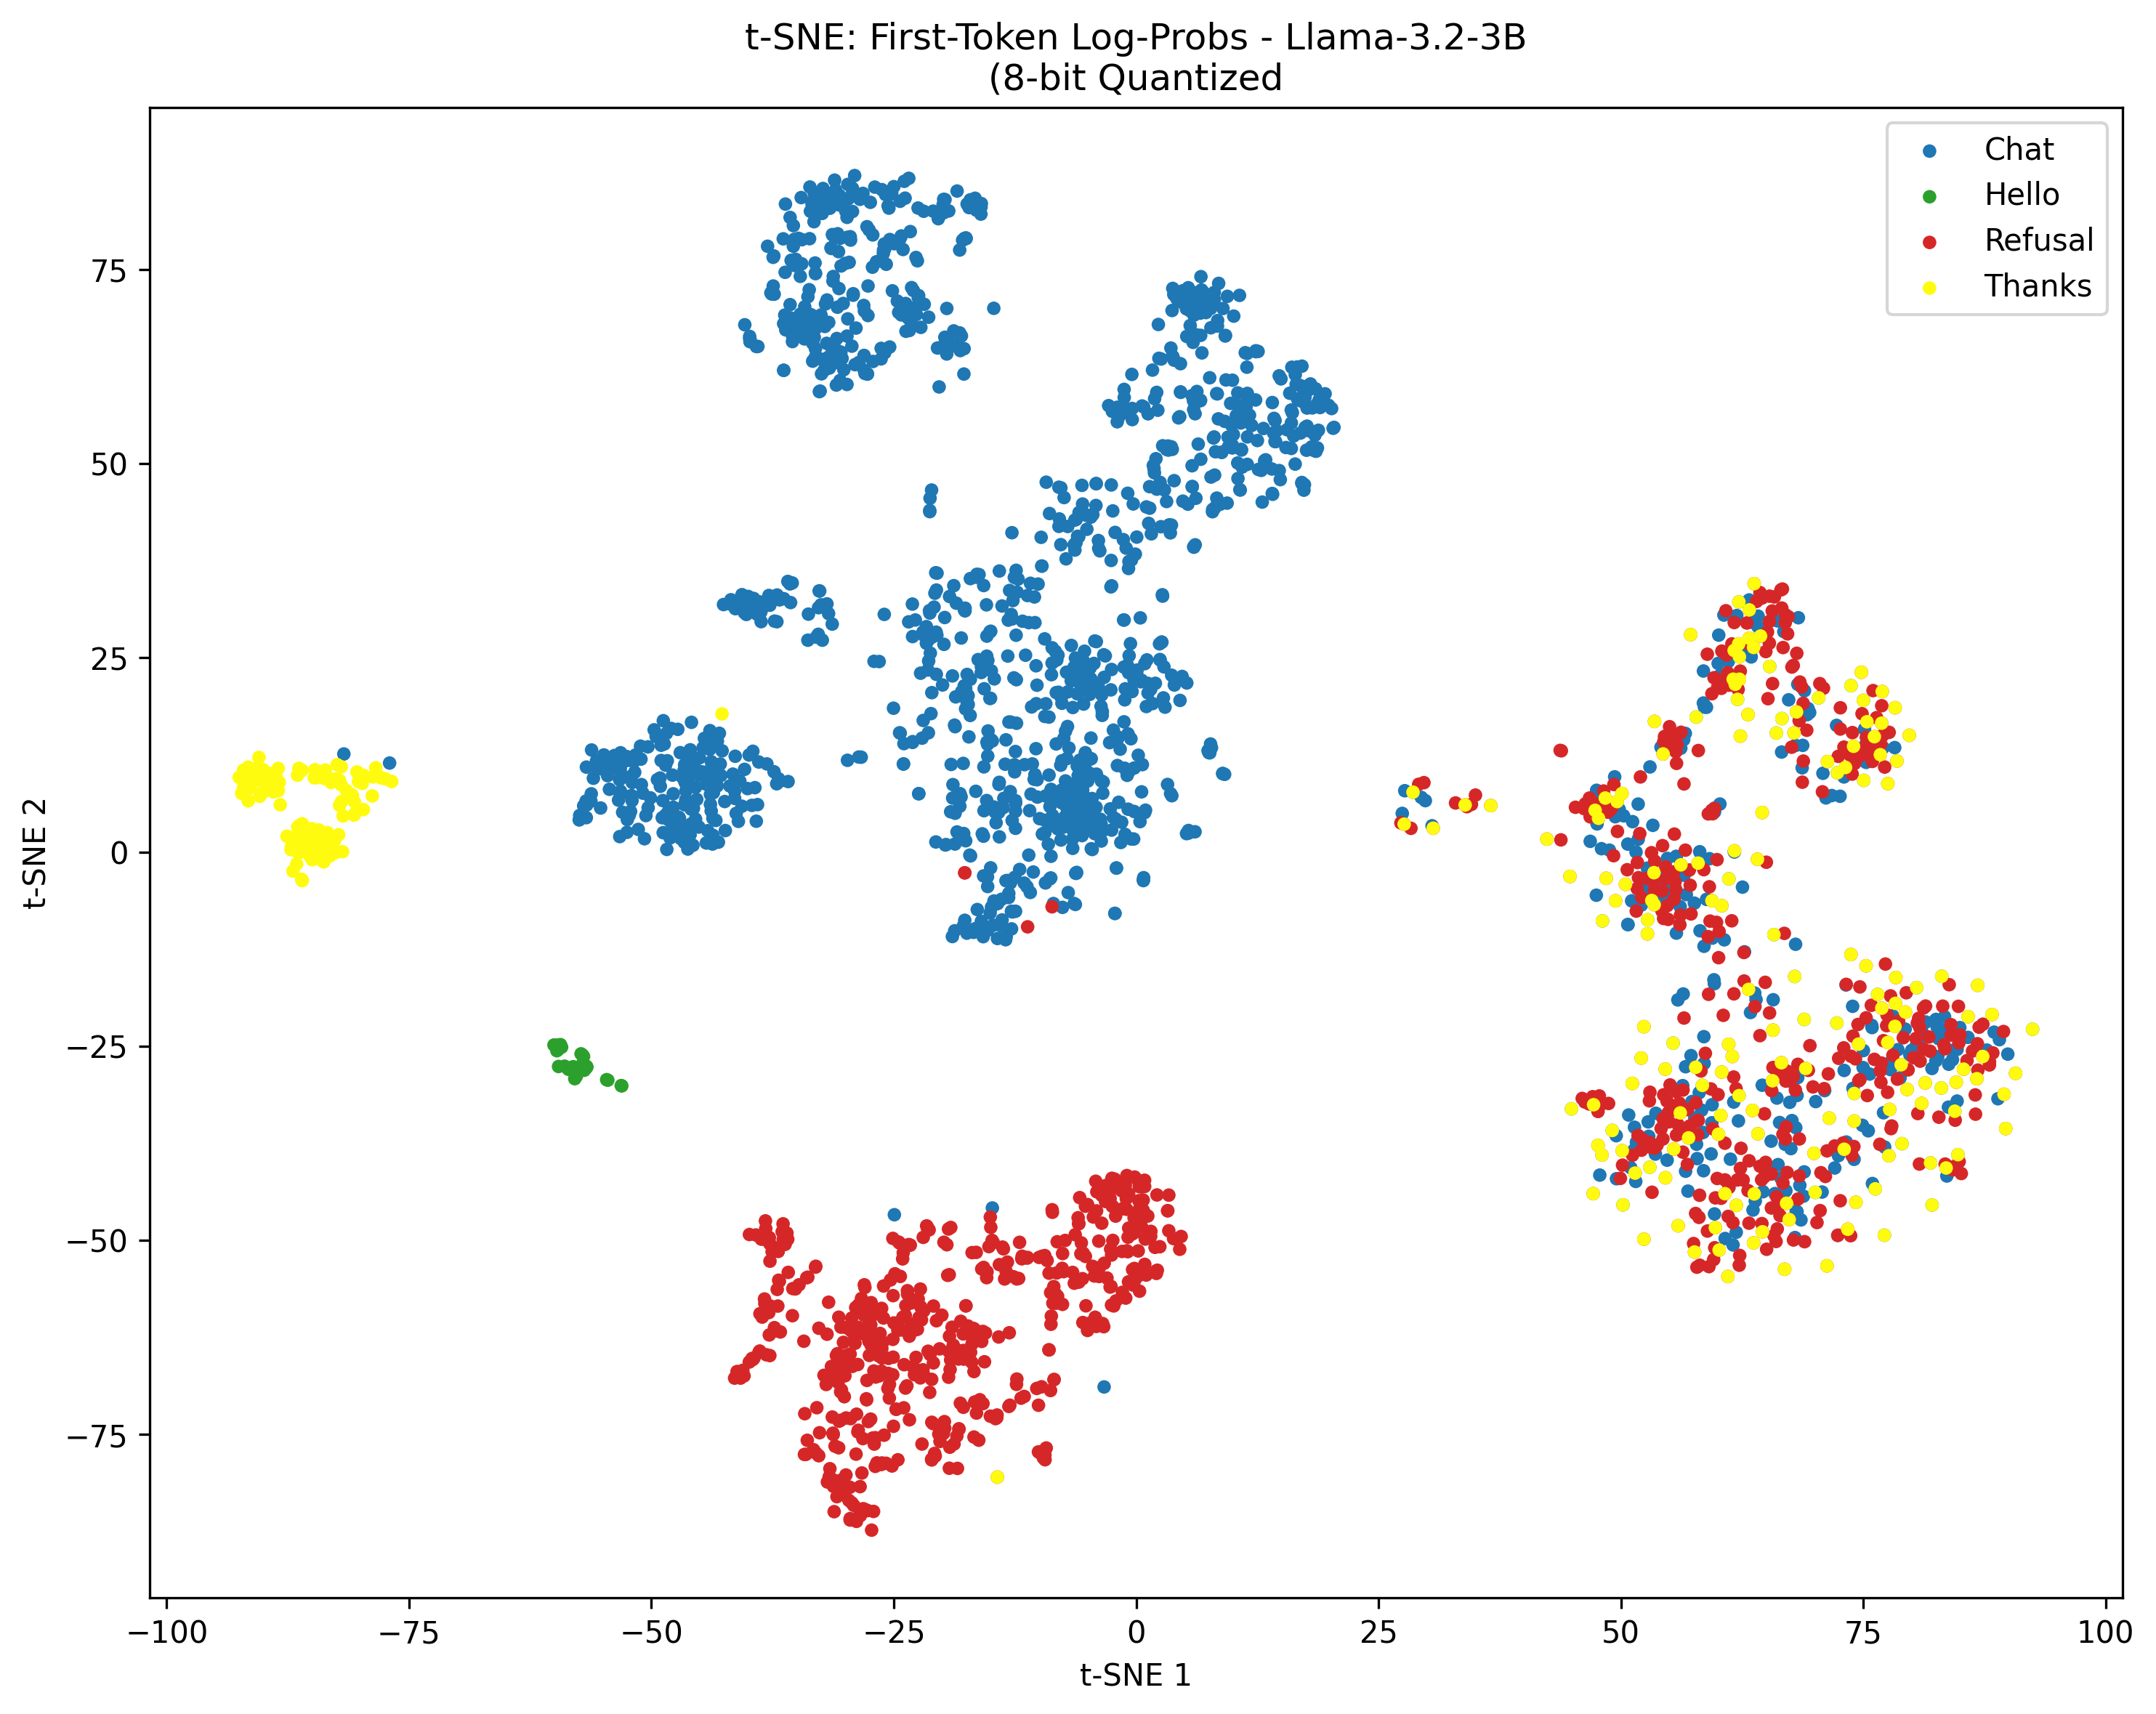
\includegraphics[width=0.7\textwidth]{tsne_Llama_3_2_3B_8bit.png}
\caption{Llama-3.2-3B: t-SNE visualization of first-token log-probabilities}
\label{fig:llama}
\end{figure}

\begin{figure}[H]
\centering
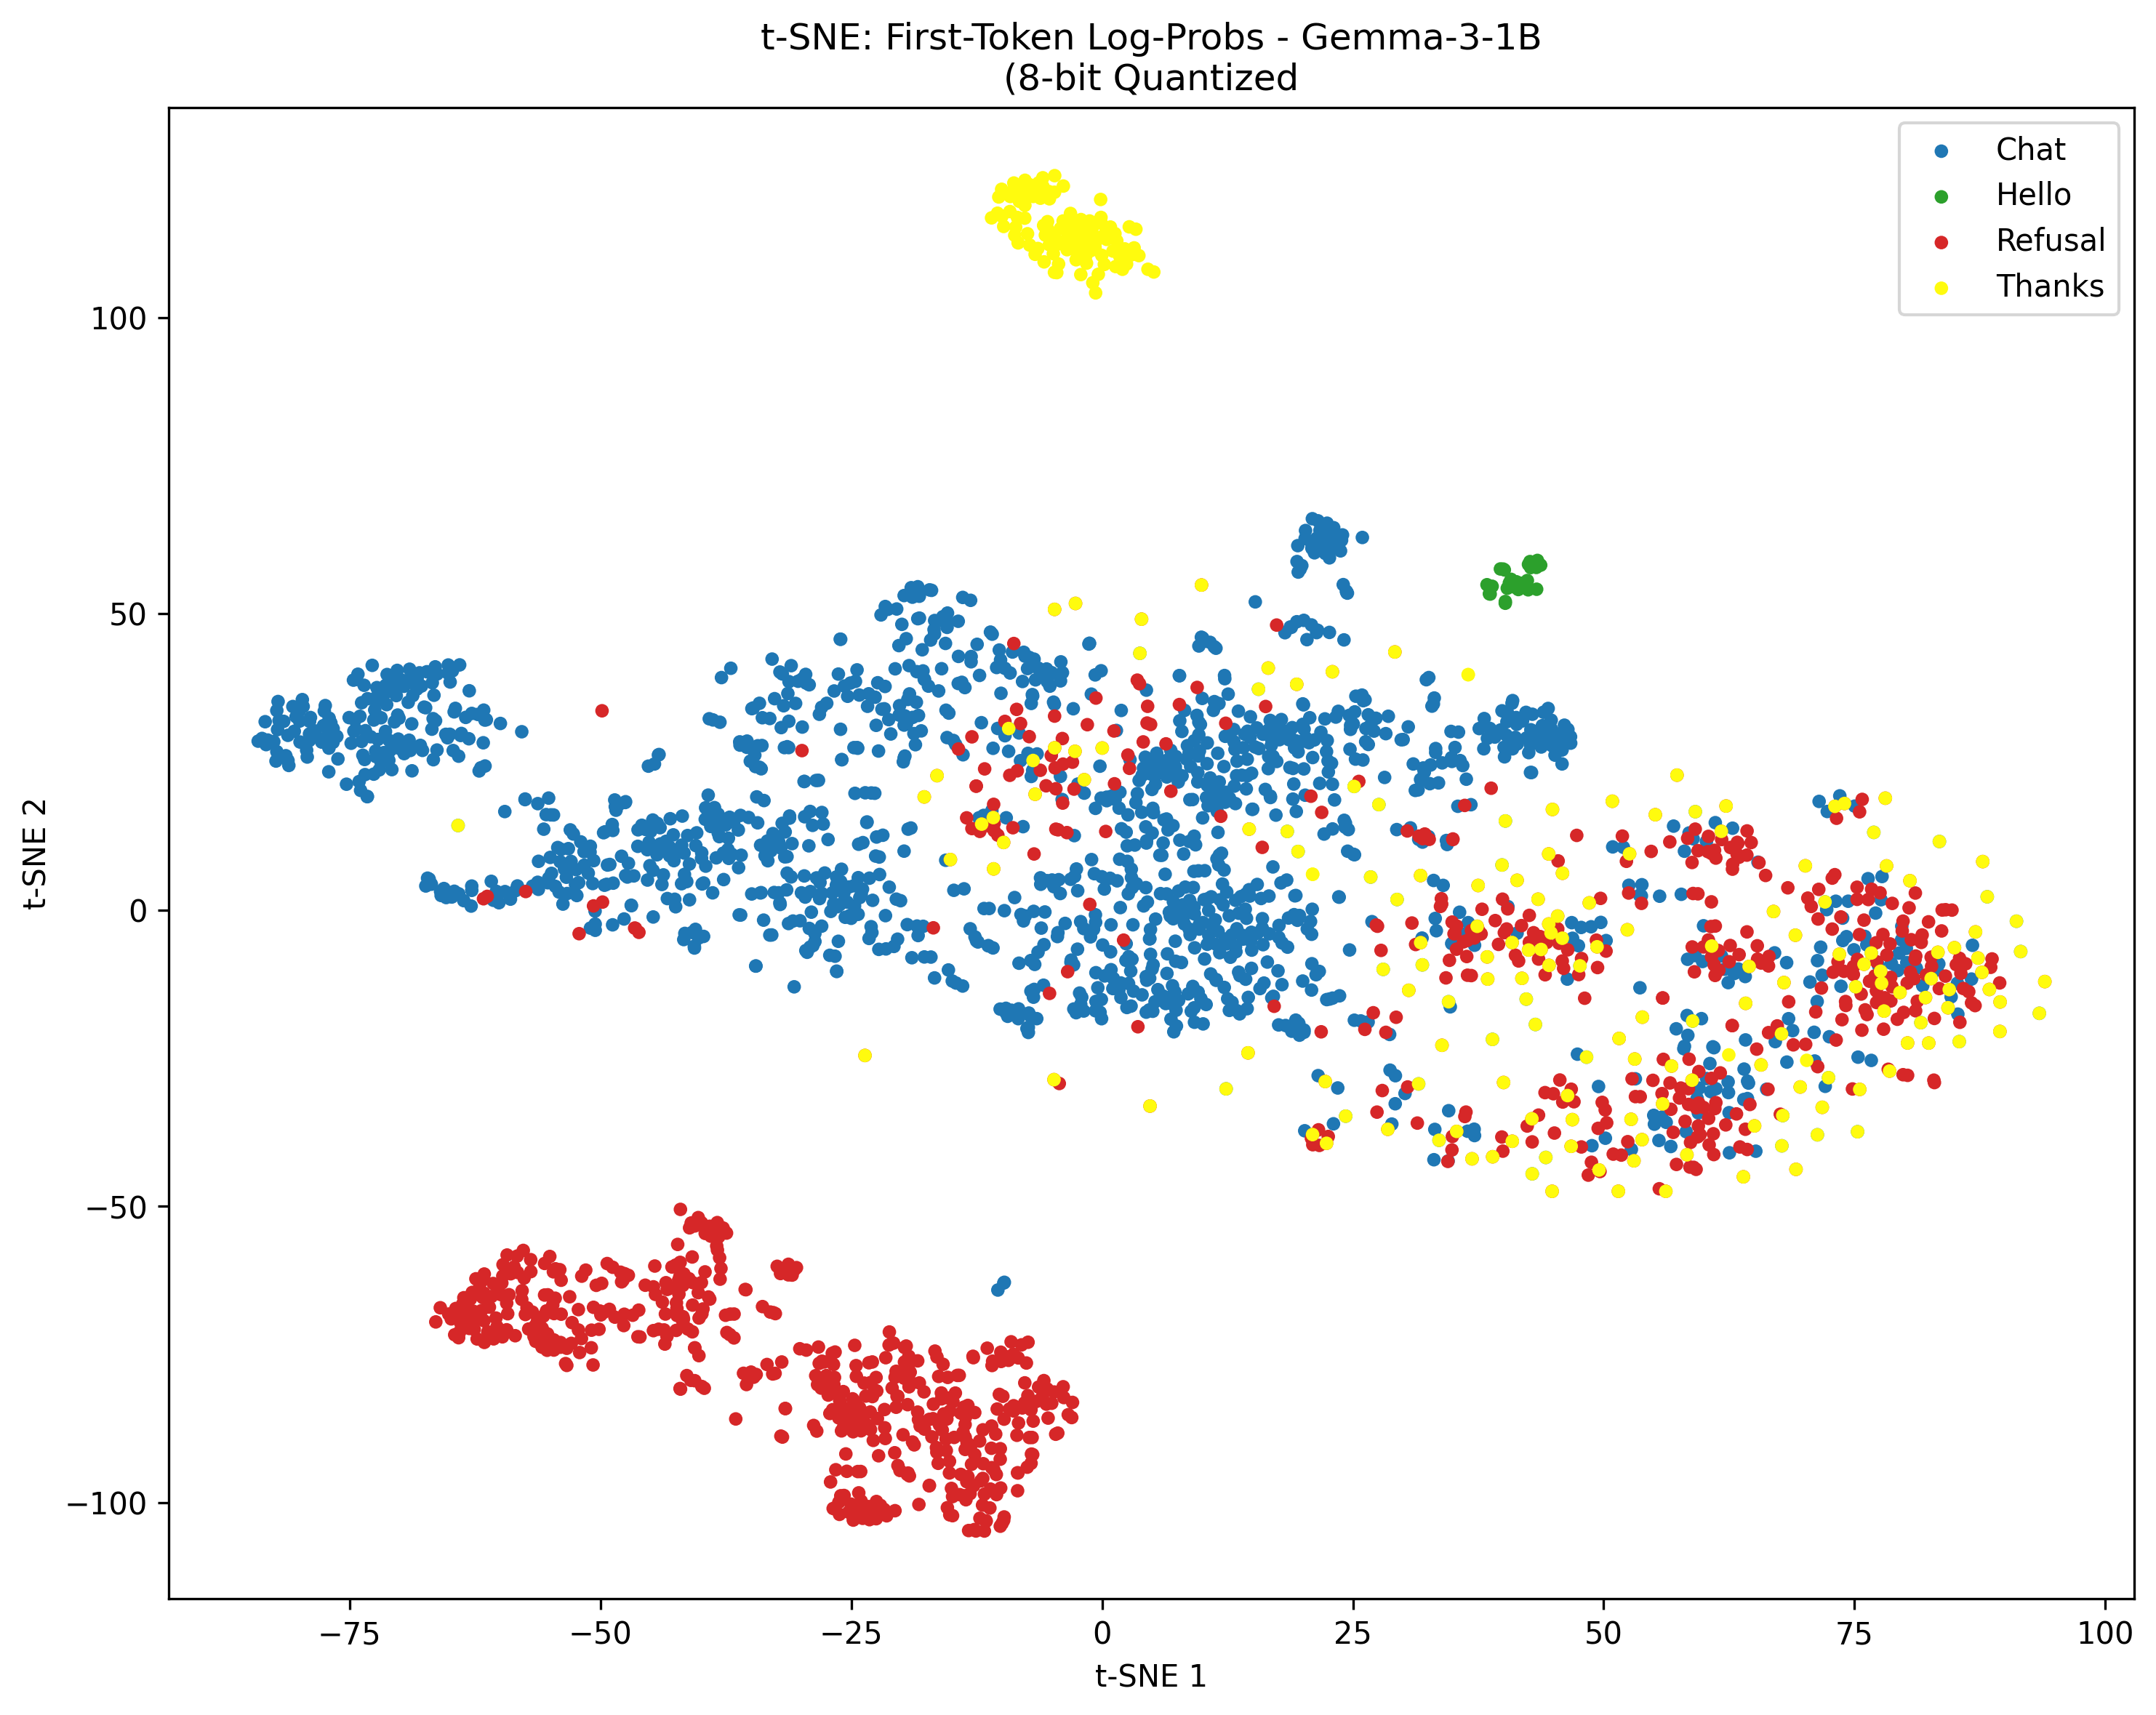
\includegraphics[width=0.7\textwidth]{tsne_Gemma_3_1B_8bit.png}
\caption{Gemma-3-1B: t-SNE visualization of first-token log-probabilities}
\label{fig:gemma}
\end{figure}

\section{Discussion}

\subsection{Key Findings}

\begin{enumerate}
    \item \textbf{First-token prediction is sufficient}: Models encode their intent before generating any output, confirming the paper's hypothesis.
    \item \textbf{Quantization robustness}: Despite 8-bit quantization, models maintain 76--79\% F1 scores, demonstrating practical viability on consumer hardware.
    \item \textbf{Generalizable approach}: The methodology works across different architectures (Qwen, Llama, Gemma).
\end{enumerate}

\subsection{Performance Gap Analysis}

The $\sim$20\% performance drop compared to the paper stems from:
\begin{itemize}
    \item \textbf{8-bit quantization}: Reduces model precision and alters log-probability distributions
    \item \textbf{Feature reduction}: Using 1,000 features vs. full vocabulary (150K+ dimensions)
    \item \textbf{Class imbalance}: Limited "Thanks" and "Hello" samples affect overall metrics
\end{itemize}

Despite these constraints, the results remain highly usable for practical refusal detection applications.

\section{Conclusion}

This work successfully reproduces the core methodology from Kainan and Zychlinski's paper on consumer hardware. By using 8-bit quantization and variance-based feature selection, we achieve competitive performance (76--79\% F1) while requiring only a fraction of the computational resources. The clear cluster separation in t-SNE visualizations confirms that LLMs encode intent in first-token log-probabilities, enabling efficient proactive detection of multiple boilerplate response types including refusals, greetings, and gratitude expressions.

\subsection{Future Work}

Potential improvements include:
\begin{itemize}
    \item Testing with full-precision models to close the performance gap
    \item Exploring alternative dimensionality reduction techniques (PCA, autoencoders)
    \item Addressing class imbalance through data augmentation or sampling strategies
    \item Extending to other intent categories beyond the four tested
\end{itemize}

\begin{thebibliography}{9}
\bibitem{kainan2025dostop}
Yuval Kainan and Shaked Zychlinski,
\textit{Do Stop Me Now: Detecting Boilerplate Responses with a Single Iteration},
arXiv preprint arXiv:2510.22679, 2025.
\end{thebibliography}

\end{document}
